% \cleartorightpage\begin{savequote}[75mm]
% In theory there is no difference between theory and practice. In practice there is.
% \qauthor{Yogi Berra}
% \end{savequote}

\chapter{In the Clinic}\label{chapter:cancer}
\setcounter{figure}{-1}
\setcounter{table}{-1}
\setcounter{section}{-1}
%\setcounter{enumiv}{-1}
\setcounter{NAT@ctr}{-1}

% \begin{figure}[t!]
% 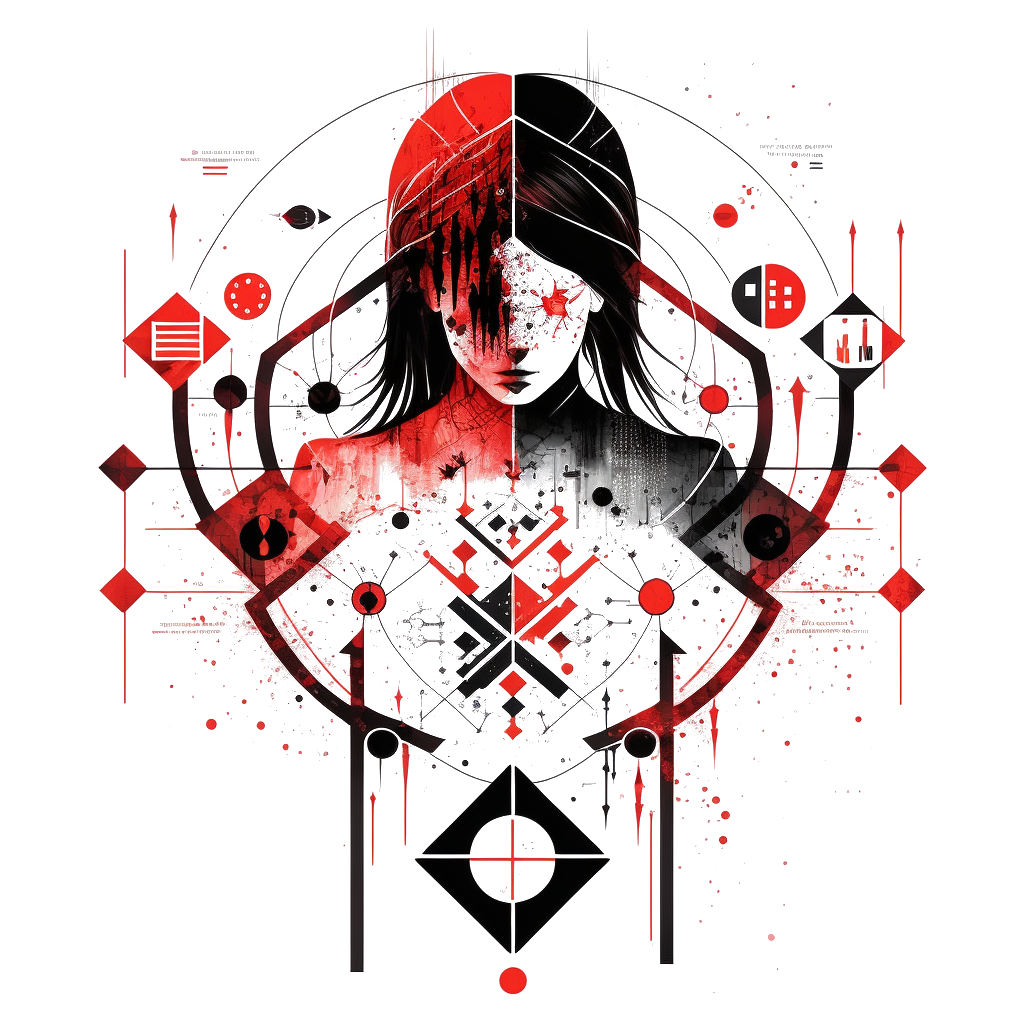
\includegraphics[height=10em]{chapters/header-cancer.png}
% \end{figure}

\setcounter{figure}{-1}
\setcounter{table}{-1}
\setcounter{section}{-1}

% In the foreword it was stated that there are no simple solutions; in this chapter we do our best to implement simple solutions for clinicians. To execute an end-to-end analysis required first integrating a manner of sensitive data retrieval within Galaxy, at which point a classical RNA-Seq analysis could be run, and subsequently a visualisation component integrated with Circos.
%
A key requirement in clinical and translational research is data privacy, necessitating the implementation of tooling for retrieving sensitive data before analysis, providing a simplified interface into shared clinical databases likes the European Genome Archive.
% we will focus on first the tooling and automation of analysis and moving towards translational medicine, before looking at a real world example of . This chapter describes the tools and pipelines we built which will enable ourselves and other bioinformaticians to put these tools and results more easily in front of Clinicians.
% Finally, Circos is a tool that makes visualisation of complex and high dimensional data easy, by utilising circular plots. Circos has a very steep learning curve and significant complexity, but at the cost of extremely flexible attractive outputs. We developed \textbf{Galactic Circos}, wrapping Circos inside of Galaxy, to increase accessibility for non-bioinformaticians, and to improve interoperability with standard analysis pipelines.

\begin{enumerate}[label=\ref{chapter:cancer}.\arabic*]
\itemsep-0.5em
\setcounter{enumi}{-1}
\item \textbf{EC-PC} We analysed the expression changes of endothelial cells and pericytes under the condition of Tumor Necrosis Factor (TNF), in two separate experiments. I completed the analysis of the RNA Sequencing data and associated visualisations confirming the up-regulation of CXCL and CCL chemokines and associated pathways.

\item \textbf{FAIR Data Retrieval for Sensitive Clinical Analysis in Galaxy} Here we discuss improvements in the connection between Galaxy and EGA, the European Genome Archive, and the development of a wrapper that more easily integrates the two data stores. I contributed to the implementation of the Galaxy integration.


\end{enumerate}
